\chapter{Evaluation}

%123456789 123456789 123456789 123456789 123456789 123456789 123456789 123456789

\label{ch:evaluation}

This chapter aims to empirically evaluate the approaches we described
in the previous chapters of this work. The structure of this chapter is as follows:
We firstly review the datasets we use for evaluation. Then we present an independent
evaluation of feature vectors (as of \autoref{ch:features}). Based on this evaluation, 
we evaluate the best performing models in end-to-end evaluation, presented
at the end of this chapter. For each of the evaluations, we also provide a description of the analysis we do.

\section{Datasets}

\label{sec:datasets}

In order to evaluate our proposed approaches, we firstly investigate the dataset we use. We work with two distinct datasets. Each dataset represent one \gls{ses}.

We restrict our experiments only on \glspl{det} of people as they are the main focus of this work. Furthermore, other classes are severely underrepresented in our datasets and number of their \glspl{det} are not high enough to provide reliable results.

The first \gls{ses} -- our first dataset -- comes from processing a single camera that captures a public square. The original recording is about 5 minutes long. The total number of \glspl{det} extracted from the recording is 181,792. We only keep \glspl{det} of people. Furthermore, we discard all the ``faulty'' \glspl{det} such as \glspl{det} of shadows, trees, or when there were multiple \glspl{det} capturing the same person in a single frame. Overall, we have left 71,732 \glspl{det} in this \gls{ses}, which we manually assigned into 274 different \glspl{iden}. We use this \gls{ses} for training \glspl{nn} for feature extraction from the \gls{det}'s images. An example from this \gls{ses} with extracted \glspl{det} can be seen in \autoref{fig:single_session}.

\begin{figure}
    \centering
    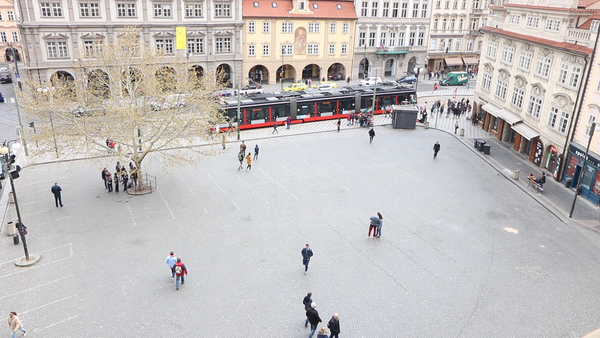
\includegraphics[width=0.48\textwidth]{img/frame_single_session_smaller.png}
    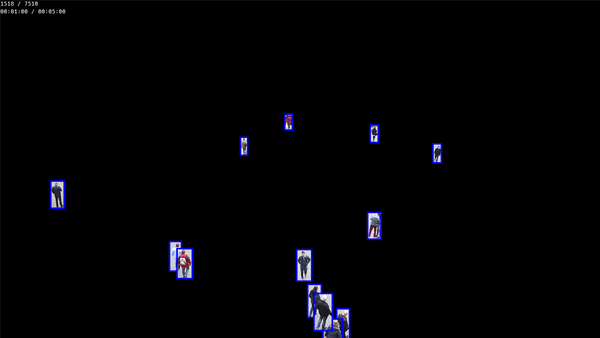
\includegraphics[width=0.48\textwidth]{img/frame_single_session_det_smaller.png}
    \caption{Frame from first session and extracted detections}
    \label{fig:single_session}
\end{figure}

We use the second \gls{ses} for actual evaluation of tested approaches. This second session is constructed from the recording of two simultaneously recording cameras. The recordings are over two minutes long. The view of the cameras partially overlap. In this session total of 147,681 \glspl{det} were extracted. Just as in the case of the previous \gls{ses}, we filter some \glspl{det} out as not usable. There remain 15,757 \glspl{det}. The worse ratio of usable \glspl{det} compared to the previous case was caused mainly by many ``faulty'' \glspl{det} of statues and lamps which were not presented in the view of the first \gls{ses}. We assigned these \glspl{det} into 52 unique \glspl{iden}. These \glspl{iden} are used as ground truth for evaluation of our approach. Examples of frames from this \gls{ses} are in \autoref{fig:double_session}.

\begin{figure}
    \centering
    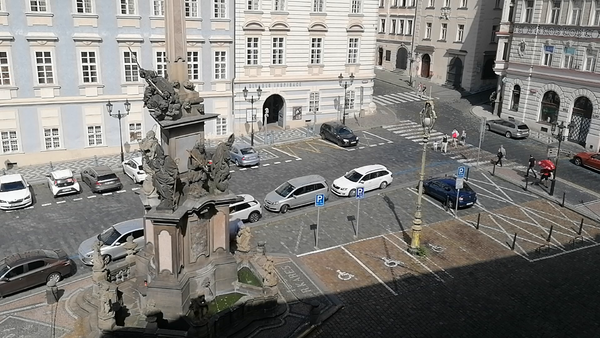
\includegraphics[width=0.48\textwidth]{img/frame_double_session_1_smaller.png}
    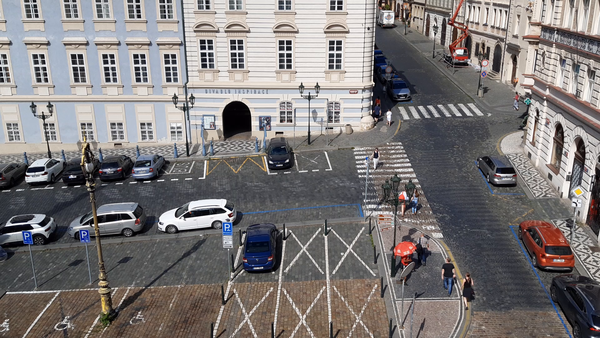
\includegraphics[width=0.48\textwidth]{img/frame_double_session_2_smaller.png}
    \caption{Frames from second session}
    \label{fig:double_session}
\end{figure}

The recordings for those two \glspl{ses} are entirely independent -- they
capture an entirely different place and were recorded at different time. This gives
us an unbiased estimation of our algorithm's quality in terms of
\autoref{eq:mla}. It would be better to evaluate our algorithm on multiple
\glspl{ses}. However, due to the technical difficulty of creating new \glspl{ses}
(especially in terms of annotating the data), we leave a more thorough evaluation
to feature work.

\section{Feature Vectors}

\label{sec:eval_fv}

Firstly, we evaluate the
quality of the feature vectors as proposed in \autoref{ch:features}. We evaluate this part purely based on how well the resulting feature vectors
separate the golden \glspl{iden} from each other. We recognize some
information is lost, as we skip the final step in this evaluation -- that is to
construct actual \glspl{iden} and compare them with the golden \glspl{iden}.
However, this preliminary evaluation is computationally less expensive, and
therefore, we may experiment with a broader spectrum of settings. We select a couple of the best performing settings and verify their usefulness later
in end-to-end evaluations.

\subsection{Measures of Quality}

To obtain comparable results, we propose several measures of quality for feature vector evaluation. We transform this problem to a standard classification task. Let us consider each pair of \glspl{det} as a single sample for classification. We aim to classify these pairs into two categories: \emph{positive} pairs where both \glspl{det} belong to the same \gls{iden}; and \emph{negative} pairs where the \glspl{det} are of distinct \glspl{iden}.

We can split the pairs to the two categories based on the golden \glspl{det} -- this sorting represents the ground truth. We can also divide the samples to the categories based on the distance: We select a threshold and for each sample (pair of \glspl{det}) we compute the distance between their feature vectors. If the distance is below the threshold we assign the pair to the positive category, otherwise to the negative category.

This allows us to sort the pairs into four standard categories used in classification tasks. First two categories -- \glspl{tp} and \gls{tn} -- represent correctly classified positive and negative samples respectively. Another category is a \glspl{fp}, which are samples that are negative but were classified as positive. Last category is \glspl{fn}, which are samples that were positive, but classified as negative.

This notation allows us to introduce two standard derived quantities -- \gls{tpr} and \gls{fpr}:

\begin{align*}
    \mathrm{TPR} &= \frac{\mathrm{TP}}{\mathrm{TP} + \mathrm{FN}} \\[8pt]
    \mathrm{FPR} &= \frac{\mathrm{FP}}{\mathrm{FP} + \mathrm{TN}}
\end{align*}

One of the characteristics of the measures is the following observation:
when we increase the threshold, the number \glspl{tp} and \glspl{fp} increases and  number of \glspl{tn} and \glspl{fn} decreases. In terms of the rates, this means that both \gls{tpr} and \gls{fpr} increases. This allows us to plot the relation between \gls{tpr} and \gls{fpr}. That is a quite common way to elaborate on the quality of \gls{ml} classifiers. The resulting plot is often called \gls{roc} curve.

Ideal classifiers would have a \gls{roc} curve going through a point
(0, 1). Such classifier with corresponding threshold would correctly
classify every input, positive or negative. We usually do not
have access to ideal classifiers. In such case we, broadly speaking,
want to come up with classifier that have \gls{roc} curve as close to
point (0, 1) as possible.

\gls{roc} curves give us a more in-depth view into the classifier.
The curve shows which trade-offs between \glspl{fp} and \glspl{fn} (or in terms
of the axis \gls{fpr} and \gls{tpr}) are possible for given classifiers.

While the \gls{roc} curve offers a quite useful evaluation of the selected approach, it is often useful to express the approach's quality as a single number. A single number is easier to compare and allows us to decide on the best performing model. To achieve this simplicity, we leverage the \gls{roc} curve. In particular, we compute the area under the curve. Generally speaking, the greater the area, the better classifier we have. We should keep in mind, however, that the single number does not fully capture the information about possible trade-offs. Therefore, we compare the \gls{roc} curves directly whenever possible.

Finally, let us note that we want to get feature vectors that help us find the same object in physically distant \glspl{det}. Therefore, we are not really interested in the distance between \glspl{det} of the same \gls{iden} from subsequent frames (as they would be matched by metadata anyways without the visual information). Therefore, for this evaluation (and drawn \gls{roc} curves) out of all positive pairs (i.e., pairs of \glspl{det} from the same \gls{iden}) we select only those which are either from different cameras or are at least 2 seconds apart.

\subsection{Evaluation of Color Histograms}

Firstly, we aim to evaluate the approaches based on the color histograms. To recapitulate, there are several basic choices
for histogram generation, we need to evaluate (please refer to
\autoref{sec:histograms} for detailed explanation):

\begin{itemize}
    \item Selection of color model
    \item Type of background filtering
    \item Number of bins of a histogram
    \item Choice of distance function
\end{itemize}

\subsubsection{Evaluation of Background Filtering}

For the evaluation of background filtering, we
aim to decide what section of the crop is important for the re-identification. The selection of background filtering should be mostly independent of
a choice of the color model and its parameters. For the experiments in this
area, we select a hue and saturation with a histogram with 8 bins in
each component (i.e., 64 bins in total).

Let us recall that we reviewed several options for background filtering. Two of the approaches has additional parameters that can be fine-tuned:

\begin{itemize}
    \item No background filtering -- no additional parameters
    \item Cropping -- total of three parameters: one parameter represent the size of the image cropped from the both, left and right size. The remaining two parameters determine how much of the image will be cropped from the top and bottom of the image. All these parameters are expressed in the percentage of the corresponding side of the image.
    \item Weighting by Gaussian -- total of two parameters: $y$ coordinate of the center of the Gaussian relative to the height of the image and the standard deviation relative to the corresponding sides of the image.
\end{itemize}

For each of these approaches, we use a grid search to find the optimal values of
these parameters. We compare the the
areas under the \gls{roc} curves as our primary metric. Furthermore, we explore some of the
\gls{roc} curves directly.
\begin{figure}
    \centering
    \def\svgwidth{\columnwidth}
    \Large
    \scalebox{0.6}{\input{img/aoc_crop_30.pdf_tex}}
    \scalebox{0.6}{\input{img/aoc_crop_20.pdf_tex}}
    \scalebox{0.6}{\input{img/aoc_crop_40.pdf_tex}}
    \caption[Area under the ROC curve for various cropping settings]{Area under the ROC curve for various cropping settings. Crop from sides is fixed in each table to the value given in the title of the plots.}
    \label{fig:aoc_crop}
\end{figure}

As we can see from the measurements in \autoref{fig:aoc_crop}, any background filtering method significantly improves the quality of the feature vectors. We note that we achieved the best performance with cropping when we 
cropped 30\% image from the left and right side, 20\% from the top and 30\%
from the bottom (although variant with 20\% achieved almost as good results). An example of such cropping can be seen in
\autoref{fig:best_cropping}. We can see that it successfully removed all the background noise.

\begin{figure}
    \centering
     \begin{subfigure}[b]{0.49\textwidth}
         \centering
         
\includegraphics[height=2.5cm]{img/0.png}
         
\includegraphics[height=2.5cm]{img/0_crop.png}
     \end{subfigure}
     \hfill
      \begin{subfigure}[b]{0.49\textwidth}
         \centering
         
\includegraphics[height=2.5cm]{img/1.png}
         
\includegraphics[height=2.5cm]{img/1_crop.png}
     \end{subfigure}
%     
\includegraphics{img/0.png} 
\includegraphics{img/1.png} \\
%     
\includegraphics{img/0_crop.png} 
\includegraphics{img/1_crop.png}
    \caption[Example of the most effective cropping]{Example of the most effective cropping -- 30\% from sides, 20\% from top and 30\% from bottom}
    \label{fig:best_cropping}
\end{figure}

\begin{figure}
    \centering
    \def\svgwidth{\columnwidth}
    \Large
    \scalebox{0.6}{\input{img/aoc_gauss.pdf_tex}}
    \caption{Area under the ROC curve for various settings of weighting by Gaussian for background filtering}
    \label{fig:aoc_gauss}
\end{figure}

In terms of weighting with Gaussian, we have achieved the best results
by offsetting the Gaussian slightly above the center of the image, to 40\%
of the height of the image, to be precise. The best setting for the standard deviation seems to be 0.2 or 0.1 of the dimensions of the image. For detailed results
of the grid search, see \autoref{fig:aoc_gauss}.

We selected the best approaches and plotted them in \autoref{fig:roc_background}. As we can see in the selected approaches gives almost identical results. For all the following experiments with the color histograms we use the cropping of 20\% from the top and 30\% from the other sides.

\begin{figure}
    \centering
    \def\svgwidth{\columnwidth}
    \input{img/background_roc.pdf_tex}
    \caption{ROC curve of various types of background filtering}
    \label{fig:roc_background}
\end{figure}

\subsubsection{Choice of Distance Function}

Another subject for our experiments is the choice of distance function. In
\autoref{ssec:used_distances} we introduced three distance functions --
Euclidean, Manhattan and Cosine. As we can see in \autoref{fig:roc_distances}
the choice of distance function have significant effect on the results.
The worst performing distance function seems to be Euclidean distance. The best one,
especially in case of lower \gls{fpr} seem to be Manhattan distance.
After all, Manhattan distance has quite straight-forward explanation in context
of histograms -- it is simply the number of pixels (relative to the size of the image) that needs to change to obtain the histogram of the second image. We use the Manhattan distance for the final experiments with the histograms.

\begin{figure}
    \centering
    \def\svgwidth{\columnwidth}
    \input{img/roc_distances.pdf_tex}
    \caption{ROC curve of various distance functions for histogram based models}
    \label{fig:roc_distances}
\end{figure}

\subsubsection{Selection of Color Model and Number of Bins}

The last parameter we need to set appropriately is the actual color model
and the number of bins per histogram. We explore several color models:

\begin{itemize}
    \item RGB model
    \item HSV model (we select only the hue component for one experiment and both hue and saturation component for another one)
    \item YUV model (we select UV components)
\end{itemize}

\begin{figure}
    \centering
    \def\svgwidth{\columnwidth}
    \Large
    \scalebox{0.7}{\input{img/model_bins.pdf_tex}}
    \caption[Area under the ROC curve for various color models and the number of bins]{Area under the \gls{roc} curve for various color models and the number of bins. The number of bins is displayed per channel. The total number of bins for HS and UV is the number of bins per channel squared, and for RGB, it is the number of bins per channel cubed. Some of the combinations were not explored as a total number of bins for these combination requires too much memory stored per each feature vector.}
    \label{fig:model_bins}
\end{figure}

For each model, we explore various numbers of bins of histograms. The areas under the corresponding \gls{roc} curves are displayed in \autoref{fig:model_bins}. Contrary to our original assumption, using the raw RGB channels yields the best results. The best variation, in particular, was with 4 bins per channel (i.e., 64 bins total).

Various phenomena can explain this results. For one, the varying lightning
conditions are not as common in our dataset as we expected. The other aspect is that many of the detected people wear either black or white clothing. This is especially complicated for the histograms with hue component. In case of black and white pixels even a small change in the actual color have dramatic impact on the hue of the pixel. See \autoref{fig:bad_hue} for the visualizations. 

\begin{figure}
    \centering
    
\includegraphics[width=3cm]{img/bad_hue_orig.png}
    
\includegraphics[width=3cm]{img/bad_hue_hue.png}
    \caption[Hue extraction from an image]{Hue extraction from an image. The image on the left is the original. The right image shows each pixel's hue. As we can see, the mono-colored black coat has various hue levels, and on the other hand, the black coat and the white background are represented by similar hue levels even though both are of entirely different colors.}
    \label{fig:bad_hue}
\end{figure}

To support this reasoning, we consider pixels with low ($< 0.2$)
value as black and non-black pixels with low saturation ($< 0.2$) as white and
assign them to separate bins for the HSV model. As we can see in \autoref{fig:black_white_roc}, this
significantly improved the performance while using HSV model. However, it still seems the best to use basic RGB decomposition.

\begin{figure}
    % \centering
    \def\svgwidth{0.9\columnwidth}
    \input{img/black_white_roc.pdf_tex}
    \caption[Effect of adding black and white bins to the hue histograms]{Effect of adding black and white bins to hue histograms. The figure shows \gls{roc} curves of histogram based approaches with RGB, hue with saturation, and hue alone decomposition with the best performing number of bins in each category. The plot shows improved performance obtained by adding black and white bins to the latter two categories.}
    \label{fig:black_white_roc}
\end{figure}

\subsection{Evaluation of Deep Learning Approaches}

In the previous section, we focused on the feature vectors based on the color models. Now, we evaluate the approaches using the \glspl{nn}. We start with the pre-trained networks as-is, as described in \autoref{sec:existing_architectures}.

\subsubsection{Use of Pre-trained Models Without Training}

% Perhaps the simplest usage of pre-trained models is to use them directly
% without any additional training. The potential in such usage is that the
% second to last layer (i.e. prior actual ``classification'' layer) has to
% contain enough of information to classify the original image. Therefore,
% we experiment whether such information is enough for our purposes.

We use ResNet and MobileNet architectures
pre-trained on the ImageNet dataset. These architectures
require the input of the fixed size. We rescale all the input \glspl{det}, as described in \autoref{ssec:resizing}. As the sizes of original bounding boxes are diverse (see
\autoref{fig:size_dist}), we can not avoid distorting the original \glspl{det}' images.
Therefore, we evaluate the performance of the networks with various input size settings.

\begin{figure}
    \centering
    \def\svgwidth{\columnwidth}
    \input{img/size_distribution.pdf_tex}
    \caption{Histogram of heights and widths of detections in pixels.}
    \label{fig:size_dist}
\end{figure}

The \gls{roc} curves for the pre-trained models are shown in \autoref{fig:pretrained_nn_roc}.
We evaluated various input sizes. In the case of MobileNet, we test
all the input sizes that are available for the architecture in the Tensorflow package. As for the 
ResNet we test a lower number of smaller sizes, mainly for its higher
complexity and poorer performance than the MobileNet.

As we can see directly from the \gls{roc} curves, the decidedly best setting for this type of the \gls{nn} annotation is MobileNet with input images resized to $128 \times 128$ pixels. Therefore, we use this setting for all subseqent experiments.

\begin{figure}
    \centering
    \def\svgwidth{\columnwidth}
    \input{img/pretrained_nn_roc.pdf_tex}
    \caption{ROC curves for pre-trained networks with different input shapes}
    \label{fig:pretrained_nn_roc}
\end{figure}

We have also experiment with different distance functions. As you can in \autoref{fig:basic_nn_roc_dist} the effect of different distance functions are rather small. Especially between Euclidean and Manhattan distance.

\begin{figure}
    \centering
    \def\svgwidth{\columnwidth}
    \input{img/basic_nn_roc_dist.pdf_tex}
    \caption{Comparison of effect of different distance functions on MobileNet with input shape 128$\times$128}
    \label{fig:basic_nn_roc_dist}
\end{figure}

\subsubsection{Fine-tuning the Pre-trained Models}

As the pre-trained models' results show, we achieve useful annotations with just using as-is pre-trained models. However, such models were trained for classification tasks, and therefore, there should be room for improvement when trained specifically on \reid{} task. We aim to verify this hypothesis by training the networks (with weights initialized as trained on classification task) on our dataset.

For the first experiment in this regard, we do not change the architecture at all. We use the architecture as-is and train it on our dataset using Triplet Loss (\autoref{sec:triplet_loss}).

\begin{figure}
    \centering
    \def\svgwidth{\columnwidth}
    \large
    \scalebox{0.8}{\input{img/training_loss.pdf_tex}}
    \caption{Training loss during the training with Triplet Loss}
    \label{fig:training_loss}
\end{figure}

As we can see from the log in \autoref{fig:training_loss} we significantly reduce the training error by this approach. However when we apply the resulting \gls{nn} on our evaluation \gls{ses} (see \gls{roc} curve in \autoref{fig:basic_nn_overfit_roc}), we see that the performance of the network significantly decreased. Furthermore, we can see that the performance worsens even after the single epoch of training. The weights are being altered too much even in a single epoch as the network's original capabilities are lost.

\begin{figure}
    \centering
    \def\svgwidth{\columnwidth}
    \input{img/basic_nn_overfit_roc.pdf_tex}
    \caption{Performance of the MobileNet at different stages of the training}
    \label{fig:basic_nn_overfit_roc}
\end{figure}

We lowered the learning rate to try to preserve the original information within the network. This proved to be the better performing approach as we managed to significantly increase the network's performance as you can see in \autoref{fig:basic_nn_lr1_roc} and \autoref{fig:basic_nn_lr2_roc}.

\begin{figure}
    \centering
    \def\svgwidth{\columnwidth}
    \input{img/basic_nn_lr1_roc.pdf_tex}
    \caption{Performance of the MobileNet -- training with learning rate $10^{-4}$}
    \label{fig:basic_nn_lr1_roc}
\end{figure}

\begin{figure}
    \centering
    \def\svgwidth{\columnwidth}
    \input{img/basic_nn_lr2_roc.pdf_tex}
    \caption{Performance of the MobileNet -- training with learning rate $2 \times 10^{-5}$}
    \label{fig:basic_nn_lr2_roc}
\end{figure}

Now, we proceed to evaluate the effect of different distance functions. This requires to train a new \gls{nn} because Triplet Loss (\autoref{eq:triplet}) depends on the choice of the distance function. In other related work we see the Triplet Loss used either with Euclidean distance or Cosine distance (or alternatively squared Euclidean distance\footnote{As the final layer of our \glspl{nn} is normalizing layer, the square Euclidean distance and cosine distance are proportional to each other: $\delta_{euclid}(\vec{x}, \vec{y}) = 2 - 2\vec{x}^T\vec{y} = 2 - 2 \cos(\vec{x}, \vec{y})$ (as the norms of input vectors are 1).}). However, we also aim to verify the usefulness of Manhattan distance, as it works well with the histogram approach.

\begin{figure}
    \centering
    \large
    
    \def\svgwidth{\columnwidth}
    \scalebox{0.75}{\input{img/lr_heatmap_euclidean.pdf_tex}}
    \vspace{1cm}

    
    \def\svgwidth{\columnwidth}
    \scalebox{0.75}{\input{img/lr_heatmap_cosine.pdf_tex}}
    \vspace{1cm}
    
    \def\svgwidth{\columnwidth}
    \scalebox{0.75}{\input{img/lr_heatmap_manhattan.pdf_tex}
    }
    \caption{Area under the ROC curve for various learning rates, distances and different number of epochs trained for MobileNet}
    \label{fig:lr_heatmap}
\end{figure}

The detailed results with different distance functions are displayed in \autoref{fig:lr_heatmap}. Changing the distance function indeed improved the performance. We obtain the best results while using Cosine distance. However, notice that even with a lowered learning rate, the best results in terms of area under the \gls{roc} curve are achieved by network trained only for a single epoch. Therefore, we split each epoch, and instead of using all 71,732 \glspl{det} in each epoch, we use only 640 \glspl{det} split among 32 batches per epoch.

With this alteration, the area under the \gls{roc} curve increases during the several initial epochs. In the case of Cosine distance, it reaches a maximum around the 40\textsuperscript{th} epoch with value 0.9145. See the plot in \autoref{fig:mini_epoch_cos}. With Manhattan distance, the maximum was reached very early and probably could be improved by further testing. However, since we achieve better results with cosine distance, we do not evaluate the Manhattan distance approach any further.

\begin{figure}
    \centering
    \def\svgwidth{\columnwidth}
    \input{img/mini_epoch_cos.pdf_tex}
    \caption{Area under the ROC curve with less samples per epoch}
    \label{fig:mini_epoch_cos}
\end{figure}

We also explore the effect of using Semihard instead of Hard Triplet Loss. The area under the curve during training is plotted in \autoref{fig:semi_hard_loss}. The Semihard option achieves the best performance so far. However, compared to the Hard loss, this increase in performance is barely noticeable. The maximum of area under the curve is 0.9161.

\begin{figure}
    \centering
    \def\svgwidth{\columnwidth}
    \input{img/semi_hard_loss.pdf_tex}
    \caption{Area under the ROC curve while using Hard and Semihard loss}
    \label{fig:semi_hard_loss}
\end{figure}

\subsubsection{Altering the Architecture}

Now, we investigate if we can improve our model by slightly altering the architecture. We add a dense layer as we discussed in \autoref{ssec:pretrained_models}. Based on findings in this section so far, we use the semihard loss with Cosine distance.

The results show that the setting where we train the MobileNet with added dense layer without freezing indeed produces the best model so far. Although, the improvement is negligible -- we achieved area of 0.9192. You can compare the actual \gls{roc} curve of this model and two models without a dense layer in \autoref{fig:final_roc}. As you can see in the plot, the performance of the network with the dense layer is worse in a very low level of \gls{fpr} (approx. below 0.1), while noticeably better for higher values of \gls{fpr}. We evaluate both networks (with and without added dense layer) in the next step of creating \glspl{iden}.


\begin{figure}
    \centering
    \def\svgwidth{\columnwidth}
    \input{img/final_roc.pdf_tex}
    \caption[ROC curves of MobileNet architecture with various alterations]{ROC curves of MobileNet architecture as-is and with added dense layer, trained with Hard and Semihard triplet selection.}
    \label{fig:final_roc}
\end{figure}


\subsubsection{Comparison with Simple Architecture}

\begin{figure}
    \centering
    \def\svgwidth{\columnwidth}
    \input{img/custom_architecture.pdf_tex}
    \caption{ROC curves the best model based on MobileNet and the best model with our architecture}
    \label{fig:custom_architecture}
\end{figure}

We also evaluate the experiments with a simple architecture presented in \autoref{ssec:custom_architecture}. We evaluated various learning rates and adjusted the size of the epoch as in case of pre-trained MobileNet architecture. The comparison between the best model of our custom architecture and the best model based on the MobileNet is in \autoref{fig:custom_architecture}. We can see that we can achieve interesting results even with a relatively simple architecture. Nevertheless, the model based on the MobileNet provides significantly better results and therefore, we use it in the subsequent experiments.

\begin{table}[]
    \centering
    \begin{tabularx}{\textwidth}{X|c|c}
          Architecture & Hard & Semihard \\
          \hline
         Basic architecture & 0.9145 & 0.9161 \\
         With dense layer, all parameters trainable & 0.9062 & 0.9192 \\
         With dense layer, only the last layer is trained & 0.8497 & 0.8477 \\
         Firstly trained the basic architecture, then added dense and continue training whole network & 0.9084 & 0.9109 \\
         Firstly trained the basic architecture, then added dense and train only last layer & 0.9048 & 0.9021 \\
         With dense layer, firstly only last layer is trained, then the whole network & 0.8461 & 0.8494
    \end{tabularx}
    \caption[Comparison of various MobileNet alterations]{Comparison of various MobileNet alterations. In a cells there are the area under the curve achived by correpsonding architecture. Each approach was evaluated with different number of epochs, only best perofmance per architecture is displayed.}
    \label{tab:final_comparison}
\end{table}

%\todo[inline]{ako to dopadlo freeze vs non freeze? ako dopadol njaprv freeze a potom unfreeze?}

\section{Trajectory Construction}

% \todo[inline]{tieto veci tu nepatria a trbea ich skratit na jeden odstavec. Uz boli povedane v kapitole 5.}
Now we proceed to trajectory construction. Unlike in the case of feature vectors, we do not conduct a thorough evaluation of various approaches at this point, as the desired result of this step is strongly dependent on the next step, which is actual \gls{iden} construction.

Nevertheless, we at least suggest some useful threshold for the quantities described in \autoref{ssec:spatial_merging} -- displacement, relative displacement and Intersection over Union. The thresholds should be set in a such manner that each resulting trajectory contains \glspl{det} only from one \gls{iden}, as we merge the trajectories but never split them afterwards. If we have a trajectory which contains \glspl{det} from two or more different golden \glspl{iden} we can never fix this ``impurity''.

This leads us to simple way to suggest suitable thresholds. For now let us consider simple displacement. We analyze the training dataset. In the dataset we look into each pair of the \glspl{det} which are no more than 0.2 seconds apart from each other and they are from different golden \glspl{iden}. For each such pair we record the displacement and consider the value as ``negative sample''. To obtain ``positive samples'' we processed all the \glspl{iden} in order of their timestamps. For any subsequent pair of \glspl{det} in each trajectory, if the pair is less than 0.2 seconds apart, we consider the corresponding value of displacement as ``positive sample''.

Then we computed the minimum over the negative samples (which gives us suitable starting point of which value to use on the testing dataset). Furthermore we counted how many positive samples are greater than the computed minimum (which gave us rough estimation of how quality the quantity is).

\begin{table}
    \centering
    \begin{tabular}{c|r|r}
         Quantity & Threshold & False over threshold  \\ \hline
         Displacement & 5.385 & 1.2938\% \\
         Relative Displacement & 0.037 & 0.4959\% \\
         Intersection over Union & 0.733 & 0.4636\%
    \end{tabular}
    \caption{Comparison of metadata quantities on training session}
    \label{tab:metadata_comparison}
\end{table}

We did this analysis for each of the considered quantities. The results are recorded in \autoref{tab:metadata_comparison}. As we can see the basic displacement has relatively low usefulness as the ratio of the positive samples above the threshold is relatively low. We shall consider the remaining two -- relative displacement and Intersection over Union in further steps.

\section{Identity Construction}

In this section, we review how well our algorithm constructs the \glspl{iden}. As a main measure of quality, we use \gls{roc} curves as in previous sections. When we evaluated the feature vectors alone, we just sorted the pairs of \glspl{det} by the distance and processes them one by one to produce \gls{roc} curve. Now, we cluster the \glspl{det} into \glspl{iden}. The decision whether the model assigns the pair of \glspl{det} to the same \gls{iden} depends also on other \glspl{det} not only on the distance between \glspl{det} in question. Therefore, we need to choose more complex approach to compute the \gls{roc} curves.

To run the evaluation efficiently we keep the compute a matrix $M$. An element $M_{i,j}$ represents how many \glspl{det} from $j$-th golden \gls{iden} were assigned $i$-th predicted \gls{iden}. Note that this is not standard confusion matrix, if you are familiar with that term. This matrix represents the distribution of \glspl{det}. Our samples for the purposes of the \gls{roc} curve are, however, \emph{pairs} of \glspl{det}. For example \gls{tp} are pairs of \glspl{det} such that both \gls{det} were drawn from the same cell of the matrix. Overall, we can compute the appropriate values for ROC curve as follows:\footnote{We actually compute number of \emph{ordered} pairs of \glspl{det}. However for the computation of \gls{tpr} and \gls{fpr} we can use ordered pairs instead of unordered pairs, as for each unordered pair there are two ordered ones}

\begin{align*}
    \mathrm{TP} &= \sum_{i,j} M_{i,j} (M_{i,j} - 1)\\
    \mathrm{FP} &= \sum_{i,j} M_{i,j} \left(\left(\sum_{j'}M_{i,j'}\right)-M_{i,j}\right)\\
    \mathrm{FN} &= \sum_{i,j} M_{i,j} \left(\left(\sum_{i'}M_{i',j}\right)-M_{i,j}\right)\\
    \mathrm{TN} &= \sum_{i,j} M_{i,j} \left(\left(\sum_{i',j'}M_{i',j'}\right) - \left(\sum_{j'}M_{i,j'}\right) - \left(\sum_{i'}M_{i',j}\right) + M_{i,j}\right)
\end{align*}

This computation allows us to keep all the values effectively updated. One merge of two \glspl{iden} together effectively translates to an update of two rows (we add the second row to the first and set the second to zeros). If we keep the sums of rows, columns, and the whole matrix separately, this allows us to keep all the values up-to-date after each marge (with just linear time w.r.t. the number of golden \glspl{iden}).

\subsection{Merging Trajectories}

For the first experiment with merging trajectories, we select the best performing \gls{nn} for feature vector generation. That is an architecture based on the MobileNet where we replace the last layer with a new dense layer and train it using Cosine distance. We create the initial trajectories using just Intersection over Union with threshold 0.9 and time window of 0.1 seconds. This threshold is a bit stricter compared to the findings in the training dataset as per 
\autoref{tab:metadata_comparison}. However, we want to make sure that for initial experiments, the trajectories will not be of mixed \glspl{iden} but that each trajectory will be a subset of golden \gls{iden}. We also have to select the threshold for the selection of representants. We choose threshold 0.1 as it allowed for effective evaluation.\footnote{Remember that smaller the threshold, more representatns will be selected which in turn requires more comparisons}


\begin{figure}
    \centering
    \def\svgwidth{\columnwidth}
    {\input{img/final_merging_initial.pdf_tex}}
    \caption{ROC curve for directly using distances from feature space and after using clustering to identities}
    \label{fig:final_merging_initial}
\end{figure}

We plot the resulting \gls{roc} curve of this approach in \autoref{fig:final_merging_initial}. For comparison we also show the \gls{roc} curve obtained by using just distances from the feature vectors -- i.e. the same approach as in  \autoref{fig:final_roc}. However in this stage we do not omit the ``easy'' pairs of \glspl{det} that were physically close together. Therefore the curve in \autoref{fig:final_merging_initial} is closer to the optimal point (0, 1) compared to \autoref{fig:final_roc} even though they represent the very same approach.

In \autoref{fig:final_merging_initial} we also see that after merging trajectories, the resulting \gls{tpr} and \gls{fpr} are worse. This is partly due to the property that we aim to leverage -- transitivity of ``belonging to a \gls{iden}''. If there are two golden \glspl{iden} which happen to have even just two \glspl{det} (one from each \gls{iden}) that are close together, the whole trajectories will be merged. This may very easily happen, especially in the case of low-quality \glspl{det}, where the poor quality causes the actual object to be unidentifiable, while the two images are actually visually similar. A few examples of falsely positive pairs of \glspl{det} are displayed in \autoref{fig:fp_pairs}.

\begin{figure}
    \newlength{\fpheight}
    \setlength{\fpheight}{3cm}


    \centering
    
    \begin{subfigure}[b]{0.3\textwidth}
         \centering
         
\includegraphics[height=\fpheight]{img/fp_0_a.png}
         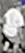
\includegraphics[height=\fpheight]{img/fp_0_b.png}
    \end{subfigure}
    \begin{subfigure}[b]{0.3\textwidth}
         \centering
         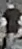
\includegraphics[height=\fpheight]{img/fp_1_a.png}
         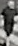
\includegraphics[height=\fpheight]{img/fp_1_b.png}
    \end{subfigure}
    \begin{subfigure}[b]{0.3\textwidth}
         \centering
         
\includegraphics[height=\fpheight]{img/fp_2_a.png}
         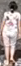
\includegraphics[height=\fpheight]{img/fp_2_b.png}
    \end{subfigure}\\
    \vspace{1cm}
    \begin{subfigure}[b]{0.3\textwidth}
         \centering
         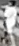
\includegraphics[height=\fpheight]{img/fp_3_a.png}
         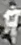
\includegraphics[height=\fpheight]{img/fp_3_b.png}
    \end{subfigure}
    \begin{subfigure}[b]{0.3\textwidth}
         \centering
         
\includegraphics[height=\fpheight]{img/fp_4_a.png}
         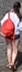
\includegraphics[height=\fpheight]{img/fp_4_b.png}
    \end{subfigure}
    \begin{subfigure}[b]{0.3\textwidth}
         \centering
         
\includegraphics[height=\fpheight]{img/fp_5_a.png}
         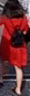
\includegraphics[height=\fpheight]{img/fp_5_b.png}
    \end{subfigure}
    \caption{Examples of falsely positive pairs}
    \label{fig:fp_pairs}
    \todo[inline]{rozsirila by som popisok}

\end{figure}
Nevertheless, we should not perceive the approach with merging trajectories as a strictly worse approach. Unless we cluster the \glspl{det} we can not query all the \glspl{det} of one given object. For example if we have just the distances of feature vectors we can, for a given \gls{det}, retrieve the other \glspl{det} in order of their visual similarity. However, this similarity drops significantly once the tracked person turns or changes her appearance in any other way. This means that the ability of drawing complete trajectories of a given person is lost.

On the other hand, approach with subsequent merging into bigger \glspl{iden} tries to mitigate this problem by keeping track of small changes and due to transitivity to keep its ability to find complete trajectories. This is however traded off by lower \gls{tpr} (or higher \gls{fpr}) which can be seen in the figure.

We can also notice, that while the \gls{roc} curve for the simple feature approach is smooth, the \gls{roc} curve of using merging is not. In particular, one can find several straight lines in the \gls{roc} curve. This is caused by the fact that once a threshold is crossed, specific \gls{iden} are merged causing jumps in \gls{tp} (if the merged \glspl{iden} were largely of the same golden \gls{iden}) or \gls{fp} (if the merged \glspl{iden} consists of \glspl{det} from distinct golden \glspl{iden}).

\subsubsection{Optimizing Parameters}

\begin{figure}
    \centering
    \def\svgwidth{\columnwidth}
    {\input{img/final_parameter_search.pdf_tex}}
    \caption{ROC for various setting for initial trajectory creation}
    \label{fig:final_parameter_search}
\end{figure}

We aim to improve this approach by appropriately changing the parameters used for the initial trajectory generation. We change the threshold for \gls{iou} during the trajectory generation, and the sliding time window size. The \gls{roc} curves for selected values of these parameters are shown in \autoref{fig:final_parameter_search}.

As you can see, these parameters for initial trajectory generation have a dramatic impact on the quality of the final clustering. We manage to improve our approach significantly. For a specific values of \gls{fpr} we even achieved higher \gls{tpr} compared to the \gls{roc} curve obtained from distances directly.

\begin{figure}
    \centering
    \def\svgwidth{\columnwidth}
    {\input{img/final_relative.pdf_tex}}
    \caption{ROC curves of identites while using relative displacement}
    \label{fig:final_relative}
\end{figure}

We also evaluated the option of using relative displacement instead of \gls{iou}. Corresponding results are displayed in \autoref{fig:final_relative}. We can produce comparable results as with \gls{iou} although using \gls{iou} still seems as a better option, hence we use it in remining experiments.

\begin{figure}
    \centering
    \def\svgwidth{\columnwidth}
    {\input{img/final_rep.pdf_tex}}
    \caption{ROC with increased number of representants}
    \label{fig:final_rep}
\end{figure}

We also shortly experiment with lowering the threshold for selecting the representants within the trajectory (which means increase the number of representants per trajectory). As you can see in \autoref{fig:final_rep} this indeed improved the model. Unfortunately, due to significantly higher computational cost, such increase in the number of representants is not suitable for practical use.

\begin{figure}
    \centering
    \def\svgwidth{\columnwidth}
    {\input{img/final_nn.pdf_tex}}
    \caption{ROC with different neural networks for producing feature vectors}
    \label{fig:final_nn}
\end{figure}

We also test whether changing the \gls{nn} would improve the results. We evaluate other approaches (network without a dense layer with hard and semihard training loss), exactly as per \autoref{fig:final_roc}. However, as we can see in the figure, the network's performance with dense layer seems to be the best option.

\subsection{Direct Identity Construction}

Lastly, we evaluate the approach where we construct the \glspl{iden} directly without a priori construction of the trajectories. Unlike in other approaches, we do not use \gls{roc} curves to evaluate this approach. The reason it would become computationally exhaustive to get all pairs. We can not sample the pairs directly and sort them based on the distance as we did in \autoref{sec:eval_fv} as the fact whether we consider two \glspl{det} to be of same \gls{iden} does not depend only on the distance between them but also on other \glspl{det}. Nor we can make use of a priori trajectory generation (as we do not use it) to make the computation of subsequent \gls{roc} curved feasible. Therefore, we select just a few hyperparameters and evaluate \gls{tpr} and \gls{fpr} just for those values.

\begin{table}[]
    \centering
    \begin{tabular}{c||c|c}
     \gls{iou} \textbackslash{} window & 0.5s & 1.0s \\ \hline \hline
     0.8 & 0.7652 / 0.3933 & 0.8005 / 0.4137 \\ \hline
     0.85 & 0.7637 / 0.3923 & 0.7997 / 0.4058 \\ \hline
     0.9 & 0.7634 / 0.3921 & 0.7624 / 0.3915 \\ \hline
     0.95 & 0.7995 / 0.4056 & 0.7796 / 0.4002 
    \end{tabular}
    \caption[Comparison of various hyperparameters for direct identity construction]{Comparison of various hyperparameters for direct identity construction. In each cell there is \gls{tpr} / \gls{fpr} for given threshold for merging using \gls{iou} and given size of sliding time window. The results correspond to the setting where trajectories are merged if two processed detections are closer than 0.3 in cosine distance.}
    \label{tab:direct_param}
\end{table}

We can review the results in \autoref{tab:direct_param}. These results were obtained with merging threshold for distance between feature vectors set to 0.3. For the other settings of the threshold the results were quite poor (\gls{tpr} below 0.4 or \gls{fpr} above 0.8). As you can see, we did not manage to improve the results compared to merging trajectories.

The main drawback of this approach is that once every \gls{det} from a \gls{iden} is removed from the sliding time window, no additional \gls{det} can be added to the \gls{iden}. To mitigate this problem, we increase the sliding window size (up to 10 seconds). This also means that the metadata becomes less useful. Therefore, we added another condition that for merging using the metadata, the \glspl{det} has to be closer together than 0.2 seconds (even though the sliding window contains \glspl{det} from 10 seconds). This increase in the window size significantly increased the time needed for processing the \gls{ses}. The obtained results for more successful settings are displayed in \autoref{tab:direct_time_window}. Unfortunately, even after these changes, we did not improve the results.

\begin{table}[]
    \centering
    \begin{tabular}{c||c|c|c}
     distance \textbackslash{} window & 5s & 10s \\ \hline \hline
     0.1 & 0.3256 / 0.0041 & 0.4496 / 0.0291  \\ \hline
     0.2 & 0.8623 / 0.2656 & 0.8651 / 0.6814 \\ \hline
     0.3 & 0.9230 / 0.8219 & 0.9232 / 0.8900
    \end{tabular}
    \caption[Comparison of various hyperparameters for direct identity construction with separate time window for spatial metadata]{Comparison of various hyperparameters for direct identity construction with separate time window for spatial metadata. The trajectories were merged only if they have \gls{iou} of at least 0.8 and were closer than 0.2 seconds or the condition for merging via feature vectors are met (as per thresholds in the table). In each cell there is \gls{tpr} / \gls{fpr} for given parameters.}
    \label{tab:direct_time_window}
\end{table}